
\subsection{{\idletime}が一般の場合}
\label{subsec:LineDifferentTimelimit}

全点の{\idletime}が等しい場合は
どの頂点も高々1人の巡査が担当するため
単純になっていたが,
{\idletime}が一般の場合は,
頂点を複数の巡査が訪問して警備する必要がある場合が存在する.
%
図\ref{tikz:multiAgentExample2}(左)の例では,
中央の{\idletime}の短い2つの頂点は2人の巡査に訪問されており,
また,全点の{\idletime}が等しい場合に反して
各巡査の最適な運行はなんらかの区間の往復であるとは限らないことも分かる.


また,
この例では左の巡査は左端の点を{\idletime}ちょうどごとに訪問しているが,
左端の点の{\idletime}から順に巡査の運行を決定することも難しい次のような例が存在する.
図\ref{tikz:multiAgentExample2}(中央)の例では,
左側の巡査は左端の点をあえてより短い周期で訪問することで全点を警邏しているが,
同じ例について,
図\ref{tikz:multiAgentExample2}(右)のように左の巡査が
左端の点の{\idletime}ぎりぎりの時間まで右の方へ動き左端へ帰る運行を行うと
2人の巡査がうまく協力できず全点の警備ができない.

\begin{figure}[htbp]
  \centering
  \begin{tabular}{ccc}
  \begin{minipage}{0.32\hsize}
    \centering
    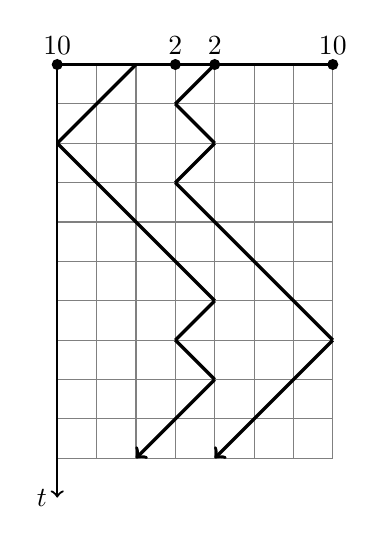
\begin{tikzpicture}
      \draw [help lines,thin,step=5mm] (0,-5.0) grid (3.5,0);
      \draw[thick] (0,0) -- (3.5,0) node [below] {};
      \draw[thick, ->] (0,0) -- (0,-5.5) node [left] {$t$};
      \fill ( 0   , 0) coordinate (c1) circle (2pt) node [above] {10};
      \fill ( 1.5 , 0) coordinate (c2) circle (2pt) node [above] {2};
      \fill ( 2.0 , 0) coordinate (c3) circle (2pt) node [above] {2};
      \fill ( 3.5 , 0) coordinate (c5) circle (2pt) node [above] {10};
      \draw[very thick,- ] ( 1.0, 0  )--(   0,-1.0);
      \draw[very thick,- ] (   0,-1.0)--( 2.0,-3.0);
      \draw[very thick,- ] ( 2.0,-3.0)--( 1.5,-3.5);
      \draw[very thick,- ] ( 1.5,-3.5)--( 2.0,-4.0);
      \draw[very thick,->] ( 2.0,-4.0)--( 1.0,-5.0);
      \draw[very thick,- ] ( 2.0, 0  )--( 1.5,-0.5);
      \draw[very thick,- ] ( 1.5,-0.5)--( 2.0,-1.0);
      \draw[very thick,- ] ( 2.0,-1.0)--( 1.5,-1.5);
      \draw[very thick,- ] ( 1.5,-1.5)--( 3.5,-3.5);
      \draw[very thick,->] ( 3.5,-3.5)--( 2.0,-5.0);
    \end{tikzpicture}
  \end{minipage}
  \begin{minipage}{0.32\hsize}
    \centering
    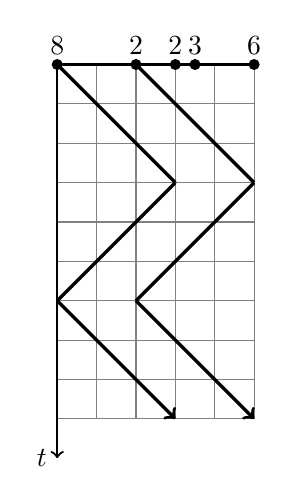
\begin{tikzpicture}
      \draw [help lines,thin,step=5mm] (0,-4.5) grid (2.5,0);
      \draw[thick] (0,0) -- (2.5,0) node [below] {};
      \draw[thick, ->] (0,0) -- (0,-5) node [left] {$t$};
      \fill ( 0   , 0) coordinate (c1) circle (2pt) node [above] {8};
      \fill ( 1   , 0) coordinate (c2) circle (2pt) node [above] {2};
      \fill ( 1.5 , 0) coordinate (c3) circle (2pt) node [above] {2};
      \fill ( 1.75, 0) coordinate (c4) circle (2pt) node [above] {3};
      \fill ( 2.5 , 0) coordinate (c5) circle (2pt) node [above] {6};
      \draw[very thick,- ] ( 0  , 0  )--( 1.5,-1.5);
      \draw[very thick,- ] ( 1.5,-1.5)--( 0  ,-3  );
      \draw[very thick,->] ( 0  ,-3  )--( 1.5,-4.5);
      \draw[very thick,- ] ( 1  , 0  )--( 2.5,-1.5);
      \draw[very thick,- ] ( 2.5,-1.5)--( 1  ,-3  );
      \draw[very thick,->] ( 1  ,-3  )--( 2.5,-4.5);
    \end{tikzpicture}
  \end{minipage}
  \begin{minipage}{0.32\hsize}
    \centering
    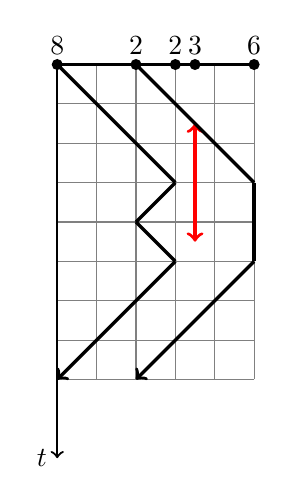
\begin{tikzpicture}
      \draw [help lines,thin,step=5mm] (0,-4) grid (2.5,0);
      \draw[thick] (0,0) -- (2.5,0) node [below] {};
      \draw[thick, ->] (0,0) -- (0,-5) node [left] {$t$};
      \fill ( 0   , 0) coordinate (c1) circle (2pt) node [above] {8};
      \fill ( 1   , 0) coordinate (c2) circle (2pt) node [above] {2};
      \fill ( 1.5 , 0) coordinate (c3) circle (2pt) node [above] {2};
      \fill ( 1.75, 0) coordinate (c4) circle (2pt) node [above] {3};
      \fill ( 2.5 , 0) coordinate (c5) circle (2pt) node [above] {6};
      \draw[very thick,red,<->] (1.75,-0.75)--(1.75,-2.25);
      \draw[very thick,- ] ( 0  , 0  )--( 1.5,-1.5);
      \draw[very thick,- ] ( 1.5,-1.5)--( 1  ,-2  );
      \draw[very thick,- ] ( 1  ,-2  )--( 1.5,-2.5);
      \draw[very thick,->] ( 1.5,-2.5)--( 0  ,-4  );
      \draw[very thick,- ] ( 1  , 0  )--( 2.5,-1.5);
      \draw[very thick,- ] ( 2.5,-1.5)--( 2.5,-2.5);
      \draw[very thick,->] ( 2.5,-2.5)--( 1  ,-4  );
    \end{tikzpicture}
  \end{minipage}
  \end{tabular}
  \caption{巡査の協力が必要な例.
    横軸を頂点の座標,縦軸を時刻として巡査の軌跡を表す.
    点の上の数値は{\idletime}を表す.
    \label{tikz:multiAgentExample2}}
\end{figure}


これらの例は,{\idletime}が異なる場合は巡査の運行を個別に決定するのは難しいということを示唆している.
しかしながら,この{\idletime}が一般の場合での{\graphLine}上の{\patProb}の困難性を示すこともできなかった.
そこで,{\idletime}より短い間隔で点を訪問しうることで運行の決定を複雑になる例が存在したことを踏まえて,
1章で定義した{\timeSpecifiedPatProbDecision}を考える.




\begin{defi}
  $S \subset \Zset \times \Nset$とする.
  任意の$(t_1, x_1), (t_2, x_2) \in S$が
  $\abs{x_1 - x_2} \leq \abs{t_1 - t_2}$
  を満たすとき,$S$は運行可能であるという.
  また,分割$\{ P_1, \ldots, P_l \}$が運行可能であるとは,
  各$P_1, \ldots, P_l$が運行可能集合となることである.
\end{defi}

任意の運行可能集合$S$に対して,
{\graphLine}上の巡査の運行$a$であって,
$S$のすべての元$(t, x)$に対して$a(t) = x$を満たす
(このとき$a$を運行可能集合$S$に対応する運行と呼ぶ)
ものが存在することは簡単に示すことができる.
よって,グラフが{\graphLine}の場合の{\timeSpecifiedPatProbDecision}は次のようにも記述できる.

\begin{timeSpecifiedPatrollingProblemOnLine}
  巡査の人数を表す正の整数$m$
  と$n$個の自然数の組$(q_i, r_i, x_i)_{ i \in \{ 1, \ldots, n \} }$が与えられる.
  集合
  $\{ (q_i k + r_i, x_i) \mid i \in \{1, \ldots, n\}, k \in \Zset \}$
  を$m$個以下の運行可能集合に分割できるか判定せよ.
\end{timeSpecifiedPatrollingProblemOnLine}

グラフが{\graphLine}の場合は順序保存運行を考えることができるのと同様に,
順序保存(運行可能)分割も考えることができる.
分割$\mathcal{P} = (P_1, \ldots, P_l)$が順序保存であるとは,
$\mathcal{P}$に対応する運行$A = (a_1, \ldots, a_l)$であって
順序保存なものが存在することであり,
これは,
$L(a,b) := \{ (t, x) \mid \abs{x - a} > \abs{t - b} \;\textrm{かつ}\; x < a \}$
として,
任意の$P_i (i \in \{ 1 \ldots, l \})$とその点$(a, b) \in P_i$について,
領域$L(a, b)$に含まれる点$(t, x)$であって
$(t, x) \in P_j (i < j)$なるものが存在しないことということもできる.

$X := \{ (q_i k + r_i, x_i) \mid i \in \{1, \ldots, n\}, k \in \Zset \}$
の任意の順序保存分割のうち一番左の集合は順序保存分割の定義から
$P_1 := \{ (t, x) \in X \mid L(t, x) \cap X = \emptyset \}$
の部分集合となる.
よって,$X$の最小の順序保存分割であって一番左の集合が
$P_1$であるようなものが存在する.
%
同様に,残りの$X \setminus P_1$の順序保存分割も再帰的に繰り返すと,
最小の順序保存分割$(P_1, P_2, \ldots, P_l)$が得られる.
このように,集合$X$の左側から貪欲に運行可能集合を取り出していく操作を繰り返すこと
により得られる分割を貪欲分割と呼び$\mathfrak{P}(X)$と書くことにする.
{\timeSpecifiedPatProbOnLine}は$\card{\mathfrak{P}(X)} \leq m$が成り立つかを判定すればよいが,
$X$は無限集合であるから分割$\mathfrak{P}(X)$を直接計算する\red{[言葉遣い?]}ことはできないように思われる.
しかしながら,この問題では$q_1, \ldots, q_n$が整数であることから
集合$X$は時刻(組$(t, x) \in X$の第1要素)について周期的であるため,
$X$の1周期分の有限部分集合を$\mathfrak{P}(X)$の一部となるように分割する計算ができれば
元の分割が可能か判定することができる.

以下では,集合$S$に対して
$S[a:b] := \{ (t, x) \in S \mid a \leq t < b \}$
と記号を定義する.
また,$T := lcm(q_1, \ldots, q_n)$とする(
$q_1, \ldots, q_n$は{\timeSpecifiedPatProbOnLine}の入力のもの).
以降は$X[0:T]$の分割を行うアルゴリズムを考えるのが目的となる.

まず,有限集合$S$の分割$\mathfrak{P}(S)$を与える{\setPartitionAlgorithm}を述べる.

\begin{setPartitionAlgorithmForTimeSpecifiedProblemOnLine}
  入力を$S$とする.
  初期値を$\mathcal{P} = \{\}$, $S' = S$とし,
  $S' \neq \emptyset$である限り1.から3.を繰り返す.
  \begin{enumerate}
    \item $P \gets
      \{ (t, x) \in S' \mid L(t, x) \cap S' = \emptyset \}$
    \item $\mathcal{P} \gets \mathcal{P} \cup \{ P \}$.
    \item $S' \gets S' \setminus P$, 
  \end{enumerate}
  $\mathcal{P}$を出力する.
  $\blacksquare$
\end{setPartitionAlgorithmForTimeSpecifiedProblemOnLine}


このアルゴリズムを用いて$X[0:T]$の分割を考える.

前述の貪欲分割の仕方で集合$S$から左端の運行可能集合
$s' := \{ (t, x) \in S \mid L(t, x) \cap S = \emptyset \}$
を取り出すときには,
定義の通り,$s'$の任意の点$(t, x)$に対する領域$L(t, x)$に$S$の点が存在しないことのみが$s'$の点の条件である.
$X$を$\mathfrak{P}(X)$へ分割するときと同じ状況で$X[0:T]$を分割するには,
任意の点$(t, x) \in X[0:T]$に対して定まる領域$L(t, x)$に含まれる$X$の点をすべて含むような,
$X$の部分集合を{\setPartitionAlgorithm}に与えればよい.


\red{[修正中]}

% この問題では,
% $X := \{ (q_i k + r_i, x_i) \mid i \in \{1, \ldots, n\}, k \in \Zset \}$
% という無限集合の分割が可能か判定しなければならないが,
% 実際には$q_1, \ldots, q_n$が整数であることから$X$の点は時刻(組$(t, x) \in X$の第1要素)について周期的であるため,
% 1周期分の有限部分集合を以下に定義する「繰り返し運行可能な」集合に分割できるかどうかさえ
% 判定すればよい.

% \begin{defi}
%   $T$を正の整数,$S \subset \Zset \times \Nset$を有限集合とする.
%   任意の$(t_1, x_1), (t_2, x_2) \in S$が
%   $\abs{x_1 - x_2} \leq \abs{t_1 - t_2}$
%   かつ
%   $\abs{x_1 - x_2} \leq \abs{T + t_1 - t_2}$
%   を満たすとき,$S$は周期$T$で繰り返し運行可能であるという.
%   また,分割$\{ P_1, \ldots, P_l \}$が周期$T$で繰り返し運行可能であるとは,
%   各$P_1, \ldots, P_l$が周期$T$で繰り返し運行可能となることである.
% \end{defi}

% 以下では,集合$S$に対して
% $S[a:b] := \{ (t, x) \in S \mid a \leq t < b \}$
% と記号を定義する.
% また,$T := lcm(q_1, \ldots, q_n)$とする(
% $q_1, \ldots, q_n$は{\timeSpecifiedPatProbOnLine}の入力のもの).

% $X$全体を$m$個の運行可能集合に分割できるとき,
% 部分集合$X[-T: 2T]$を
% 後で述べる{\setPartitionAlgorithm}で分割すると,
% 大きさ$m$以下の分割 $\mathcal{P} = \{ P_1, \ldots, P_l \}$ が得られる.
% %
% 一方,
% $X[-T: 2T]$を
% {\setPartitionAlgorithm}で分割した結果が
% $\{ P_1, \ldots, P_l \}$となるとき,
% $\{ P_1[0:T], \ldots, P_l[0:T] \}$は$X[0:T]$に対する
% 分割でありかつ周期$T$で繰り返し運行可能となる.
% よって,
% $X[kT:(k + 1)T]$を$X[0:T]$と同様に分割したものを
% $C_k := \{ C_{k1}, \ldots, C_{kl} \}$とすると,
% $A_i := \bigcup_{k \in \Zset} C_{ki}$として
% $\mathcal{A} := \{ A_1, \ldots, A_l \}$は
% $X$の運行可能分割となる.

% 以上から,$X$を$m$個の運行可能集合へ分割できるかどうかは,
% $X[-T:2T]$を{\setPartitionAlgorithm}により分割した結果$\mathcal{P}$が
% $\card{\mathcal{P}} \leq m$を満たすかどうかで判定できる.

% \begin{setPartitionAlgorithmForTimeSpecifiedProblemOnLine}
%   入力を$S$とする.
%   初期値を$\mathcal{P} = \{\}$, $S' = S$とし,
%   $S' \neq \emptyset$である限り1.から3.を繰り返す.
%   \begin{enumerate}
%     \item $P \gets
%       \{ (t, x) \in S' \mid x - x' \leq \abs{t - t'} \;\textrm{for any}\; (t', x') \in S' \}$
%     \item $\mathcal{P} \gets \mathcal{P} \cup \{ P \}$.
%     \item $S' \gets S' \setminus P$, 
%   \end{enumerate}
%   $\mathcal{P}$を出力する.
%   $\blacksquare$
% \end{setPartitionAlgorithmForTimeSpecifiedProblemOnLine}

% {\setPartitionAlgorithm}は,
% 有限集合$S$を入力として,
% $S$の最小の運行可能分割であって「順序保存」なものを出力する.
% 運行可能分割が順序保存であるとは,
% その分割から順序保存運行が生成されることである.
% {\graphLine}における順序保存運行の存在と同様に,
% 任意の$S$に対して最小の運行可能分割であって順序保存なものが存在する.
% $\{ (t, x) \in S' \mid x - x' \leq \abs{t - t'} \;\textrm{for any}\; (t', x') \in S' \}$
% は,$S'$の順序保存な運行可能分割において一番左にあるもののうち最大のものである.

